\documentclass[English]{dicomopapers}

\usepackage[dvips]{graphicx}
\usepackage{latexsym}
\usepackage{mathtools}
\usepackage{url}
\usepackage{tabu}
\usepackage{booktabs}
\usepackage{multirow}
\usepackage{graphicx}
\usepackage{CJKutf8}
\graphicspath{{.figures/}}
\graphicspath{{figures/}}
\newcommand\newblock{\empty}

\def\Underline{\setbox0\hbox\bgroup\let\\\endUnderline}
\def\endUnderline{\vphantom{y}\egroup\smash{\underline{\box0}}\\}
\def\|{\verb|}

\begin{document}

\title{A Research on Big Data and AI Analysis Algorithm Optimization Using GPUs}

%\affiliate{IPSJ}{Information Processing Society of Japan}
%\paffiliate{DICOMO}{DICOMO2018}
\affiliate{SOICT}{University of Tokyo, Graduate School of Information Science and Technology, Social ICT Center}
\affiliate{CS}{University of Tokyo, Graduate School of Information Science and Technology, Department of Computer Science}

\author{TRAN VAN SANG}{CS}
\author{KOBAYASHI RYOUSUKE}{SOICT}
\author{YAMAGUCHI RIE}{SOICT}
\author{NAKATA TOSHIYUKI}{SOICT,CS}

\begin{abstract}
With the significant increase of computer performance, in recent years, many complex human-like tasks have been resolved by computer software in reasonable time. These tasks include visual object recognition, speech to text interpretation, human face authentication, etc\ldots. However, computer performance is going to reach the limit as the CMOS transistor size near the limit. On the other hand, the amount of data which need to be processed is incredibly growing up under Internet of Thing, Industrialization 4.0, social network era~\cite{lohr2012age}, which leads to the demand of higher scalability on current Big Data, AI analysis algorithms. Our research investigated on finding scaling solution for Big Data, AI analysis problems. The whole development is composed of 2 phases: acceleration by GPU and distributed computing application. This research focuses on the former topic. A real-world dataset was used in this research to achieve more real-life optimization and model evaluation result.
\end{abstract}

\maketitle

%1
\section{Introduction}
In recent years, with the explosion of internet and mobile evolution, internet service is becoming bigger and bigger in terms of system complexity and user volume. Concerning user privacy and credentiality, internet service providers never want to give credential to wrong user. An obvious and canonical method is to use a combination of secret password and unique user identification. However, this becomes a burden for service users to remember their password on each service. There also is a trade-off between remembering convenience and security level when choosing a password. User behaviour of sharing password among multiple services raises the password leaking risk. Recently, there is a new way to give credentiality using Lifestyle Authentication. Lifestyle Authentication is a brand new authentication method which makes use of user auxiliary information rather than user id and password combination~\cite{weko_175884_1}. Auxiliary information can be user location paired with system access timestamp, user daily access pattern, etc\ldots. With this authentication method, a system can identify and authorize a user without requiring him/her doing any procedure explicitly. Yamaguchi Laboratory, Social ICT Center, University of Tokyo, is investigating this authentication method, and MangaONE is one of candidates for their research.\newline
MangaONE~\cite{mangaone}, one of biggest Manga providers in Japan, with very large number of users and high frequent daily access. Researchers in Yamaguchi Laboratory, Social ICT Center, University of Tokyo, and we are using MangaONE system log information for authentication application, by building a model to distinguish an user's behavior from all others'. Machine Learning, which recently attracts much public attention and many giant corporations' attention, is one of computer science fields which can be able to be applied on unstructured and multiple features data due to its ability to mimic human like task by computer. There are also many Machine Learning models which can be applied to this authentication problem. For example, Multilevel Hypergraph Partitioning~\cite{karypis1999multilevel}, Random Forest, Decision tree, k-Nearest Neighbourhood, k-means. R. Kobayashi~\cite{kobayashi1} used Random Forest model to train one model for each user with negative samples randomly chosen from all others. Beside plenty choices of models and acceleration techniques, another topic which data analysts usually care about is programming language. R is one of the most popular language for data analyst in recent years because of its high interactivity, user friendly syntax and flexible data manipulation but its speed is sometimes problematic.\newline
  With machine learning's recent large scale research community and investment, it has been improved significantly. Basic models with basic algorithms nearly reach their best performance in single machine while input data size keeps increasing with tremendous pace. As a result, there is a need to horizontally scale up the algorithm via GPU acceleration or distributed computing. Horizontally scaling up an application means to divide the application into many smaller tasks in order to execute them in multiple machines in parallel in a network such as distributed system, or execute them with GPUs. According to CRAN Task View~\cite{cran_task}, there are many GPU libraries to speedup R's standard application, such as gputools, gpuR,\ldots. However they almost support only basic matrix and vector manipulation and lack Machine Learning model training using GPUs. Gputools is a rare library that trains General Linear model using GPU but it only supports single precision number. R. Kobayashi~\cite{kobayashi1} provided very efficient model to identify user with relatively low false rate but his model requires training one model for each individual. This reduces overall scalability of the solution. His model also ignores majority of input data when training each model because taking all negative data will bias the model and the result predictor will become an one-way negative predictor.\newline
	Our research investigated on using one single model to distinguish any user behaviour in database. Then afterward, we integrated GPU into the standard implementation to speedup the critical part of the training algorithm. In acceleration phase, we chose General Linear model to optimize because of its high correction rate and reasonable resulted predictor. The optimization accelerates the algorithm bottleneck portion around twice.\newline
	Our paper is composed of 3 sections. In the next section, after describing test environment, data sanitization and model choice, we explain our improvement using GPU in detail. In following section, we show model training and optimization result with summary. Because of time margin, we could not implement all optimization strategy. Thus, in the last section, there will be discussion on future development plan in terms of modeling and optimization.

\section{Methodology}
This section is composed of 3 subsections: data manipulation, model selection, and optimization. Data manipulation subsection describes input raw data, data filtering, how to convert data into feature vector before explaining how to generate false samples for supervised learning model. Model selection subsection is subdivided into unsupervised learning, supervised learning models, and other approaches discussion. Unsupervised learning deals with k-means, k-nearest neighbor, random forest, decision tree, neural network, linear discriminant analysis, and a very promising graph based Multilevel Hypergraph Partition approach. Before mentioning some visualization techniques in other approaches subsection, the main approach of this research, General Linear model, is then described in supervised learning subsection, together with Decision Tree model. Following model selection subsection is optimization where there is discussion on how GPU optimization is conducted and several benchmark tools and techniques will be described.
\section{Data manipulation}
In our research, we ran benchmark on a dedicated machine equipped with CPU AMD Ryzen Threadripper 1950X 16-Core Processor 2.2GHz, 128GB of Memory, NVIDIA GeForce GTX 1080Ti 11GB Memory\@. Original raw data includes 41,638,144 records of user manga reading log information with 8,502 manga chapters over 49,261 users in nearly 9 months between 2014 December 18, 19:18:47 JST and 2015 September 10, 03:56:20 JST\@. Each record contains 3 elements: user's system unique user id, chapter id read by user and timestamp of the reading. System unique user id is arbitrary and unique number generated by system and does not contain any user private information.\newline
First, data was filtered by removing all data of first day and last day because these days' log information may not be completed and their portions are small enough to not affect overall performance. Next, all records of same user on same hour of same day were aggregated into one record with a new label representing number of records, i.e.\ number of the user's reading on specific hour in specific day. Then, week day of the reading was also calculated into integer values between 0 and 6, with Sunday be 0, Monday be 1,\ldots and Saturday be 6. Finally, we came up with data table of 4,532,246 records, each record having 26 data features and 1 label feature as described in Table~\ref{table:db_description}\newline
\begin{center}
  \begin{table}
    \caption{Data Table for Training Model}\label{table:db_description}
    \begin{tabular}{|p{\columnwidth / 5}|p{\columnwidth / 5 * 4}|}
      \toprule
      \textbf{Feature} & \textbf{Description} \\
      \midrule
      {User id} & {User's system unique id. There are 49,261 users in total} \\
      \midrule
      {Weekday} & {Sunday: 0, Monday: 1, \ldots, Saturday: 6} \\
      \midrule
      \multirow{2}{*}{\(h_1, h_2, \ldots, h_{24}\)} & {Number of reading in an specified hour in a specified day} \\
      & {For example: h1 feature presents number of reading from 12AM before}\\
      \bottomrule
    \end{tabular}
    \newline
  \end{table}
\end{center}
Due to the fact that finer timestamp division, for example combining data into 30 minutes chunk instead of 1 hour, is believed to make higher quality predictor, in future research, various timestamp division should be consider to achieving the best prediction rate. Moreover, time division does not need to be uniform, it can be any pattern depend on their particular characteristic. For example: sleeping hour (from 11PM last day until 6AM), commuting hour (from 6AM to 8AM), working hour (from 9AM to 12AM and from 1AM to 5AM), lunch hour, etc\ldots. This shows very high potential for future improvement of this approach.\newline
On weekday field, because of its categorical type, it is the best if this field is encoded into vector of 7 binary elements presenting 7 days in a week with one and only one element be TRUE to appoint its representing weekday. In this research, we kept them as its numerical value to simplify the model.\newline
At current development, the best way is likely to treat user id feature as numerical value because of its large domain.\newline
This data design may raise a question on why chapter id feature was removed. In fact, if chapter was a static feature, in other words, if it never changed by time, it would have been considered to be a component of the model. Moreover, chapters are also grouped into 207 groups by theirs manga with many useful additional data. This has potential to reduce input data size while still preventing loss of information on what user read. However, if chapter information is included in the model, by time user might lose his/her interest in reading some chapters, his/her reading behaviour with the chapter he/she read becomes variate, and the trained model will be invalidated.\newline
For supervised learning model training purpose, the next step in the data process is negative sample generation. User id and weekday were uniformly randomized from their domains. All newly generated values' label are false. However, with uniform generator for remaining 24 features of number of reading, Decision Tree model produced a predictor that can correctly predict 99.31\% test samples, which implies a bad data generation rather than leveraging the training model's performance. Hence, we investigated new way to generate number of reading to generate data more likely to existing data. Because all users usually do not read manga on every hour, there should be more zero value in these 24 features. In order to do this, firstly, number of total reading of each user was investigated. Figure~\ref{fig:total_hist} 2 shows this value histogram.\newline
\begin{figure}[ht]
  \vspace*{-1cm}
  \centering
  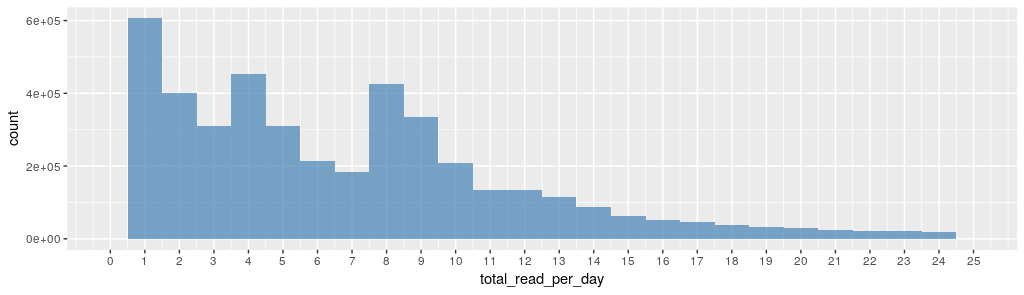
\includegraphics[width=\columnwidth,natwidth=1024,natheight=295]{total_hist.png}
  \caption{Total number of reading per day of each user histogram}\label{fig:total_hist}
\end{figure}
\newline
Figure~\ref{fig:total_hist} illustrates that total number of reading in a day regardless user more concentrates at lower values from 1 to 7 times, then concentrates again at 8 before slightly dispersing until infinity. To achieve same total reading per day distribution on newly generated data, total number of reading of each new record S firstly randomized from set of all total number of reading in original data regardless of the user. Next, 23 numbers \(k_1, k_2,\ldots, k_{23}\) were uniformly randomized between 0 and S with replacement. With \(k_0 = 0, k_{24} = S\), 24 features \(h_1, h_2,\ldots, h_{24}\) then calculated by\newline
\begin{center}
  \(h_i = k_i - k_(i - 1)\) with \(i = 1\ldots24\)\newline
\end{center}
	Number of negative samples generated is exactly same as number of positive samples. After negative sample generation, there was 9,064,492 records in total. In model evaluation, 70\% of them were used to train the model and 30\% were for testing. In optimization phase, 100\% data was used for better comparison result.
\section{Model selection}
\subsection{Unsupervised approach}
Following unsupervised approaches only consider positive samples with \texttt{label} feature removed.\newline
The very first approach was unsupervised k-mean model. All samples were grouped into \(k\) clusters of interested to minimize each data group's variance based on their Euclidean vector distance. Modified version of gap statistics in~\cite{RSSB:RSSB293} was used to identify the \(k\), number of clusters. Found number of clusters was 7. Figure~\ref{fig:gap_stat} shows gap statistic value of variate \(k\) values. Statistic value show how much sum of squared distance within cluster clustering gains by increase number of clusters from \(k - 1\) to \(k\). In gap statistic, \(k\) value should be chosen with their highest gap statistic value. However, from Figure~\ref{fig:gap_stat}, gap statistics seem to increase consistently. We heuristically chose \(k = 7\) because of the slight decrease of gap statistic value when \(k\) goes from 7 to 8. Subsequently, clusters were evaluated by calculating how many clusters each user has their samples belong to in average. Evaluated number was 4.7 clusters over total 7 clusters. In other words, each user has samples presenting more than half of all clusters, while at most one or two clusters had been expected for k-means model to be adopted.\newline
\begin{figure}[ht]
  \vspace*{-2cm}
  \centering
  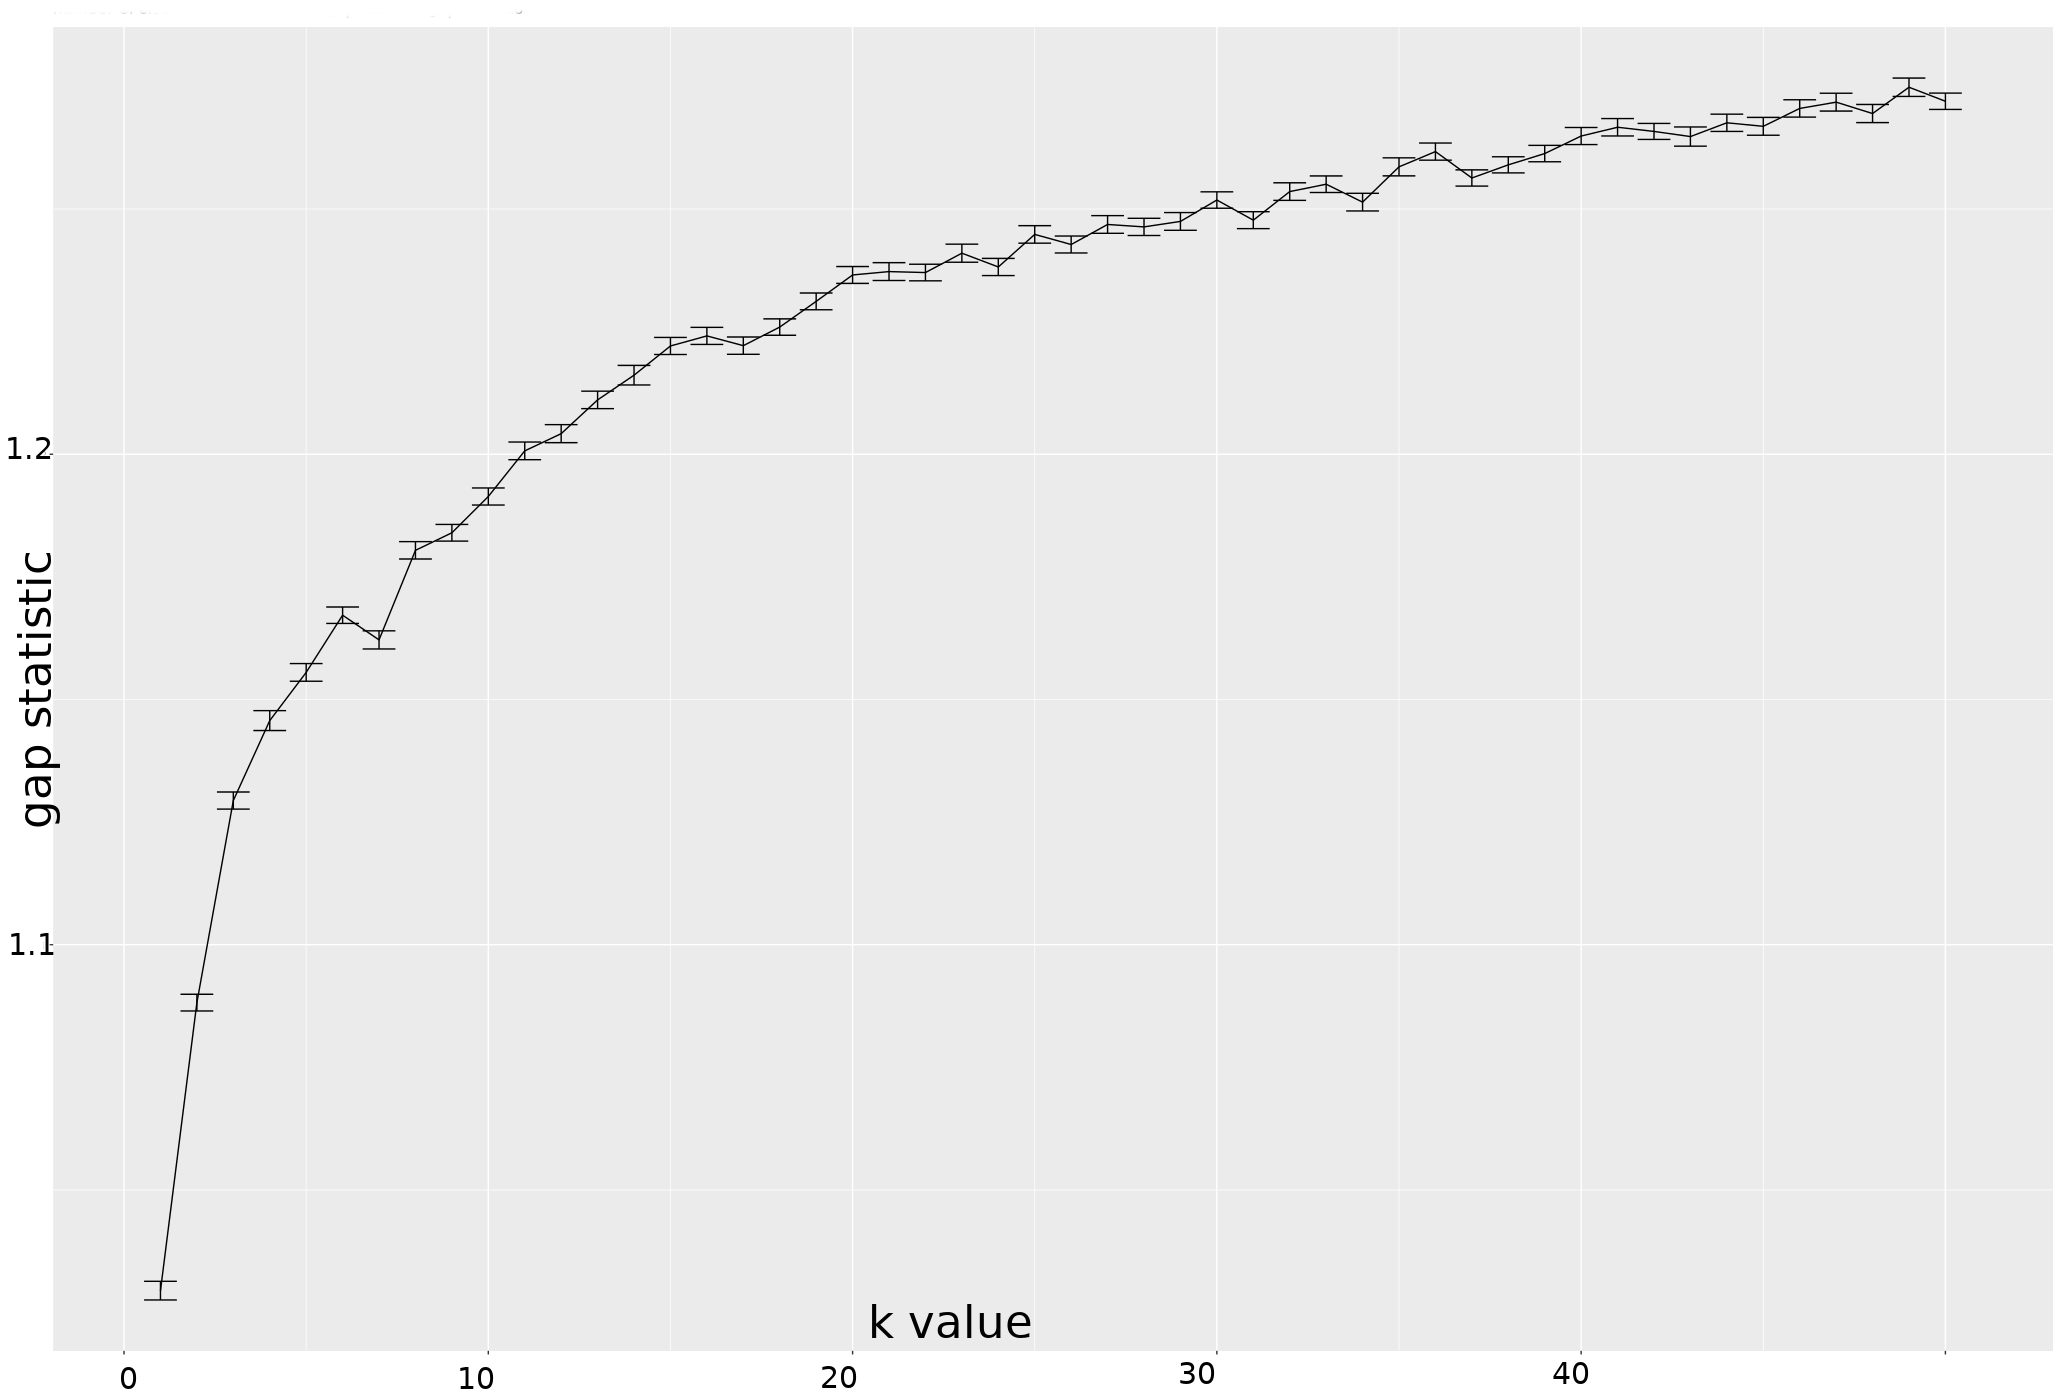
\includegraphics[width=\columnwidth,natwidth=2060,natheight=1398]{gap_stat.png}
  \caption{Gap statistics of multiple \(k\) value}\label{fig:gap_stat}
\end{figure}
\newline
 Similar to k-means, k-nearest neighbor model was also applied by finding most \(k\) nearest records from training data for each record in testing data. Dominated user in set of \(k\) nearest neighbors is used to label test data. Unlike k-means model, k-nearest neighbor can use any of distance function. Figure~\ref{fig:knn} illustrates error rate of this model with variate minkowski distance, which points out that this model cannot make correct prediction of more than 4\% of test samples.\newline
\begin{figure}[ht]
  \vspace*{-2cm}
  \centering
  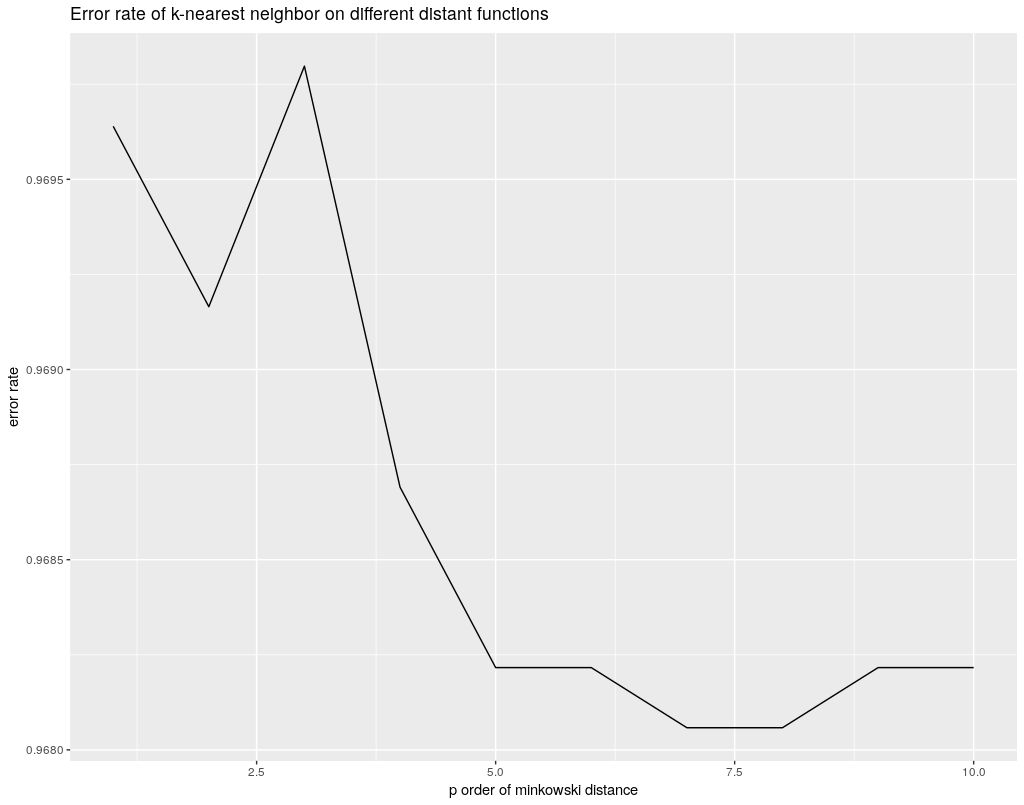
\includegraphics[width=\columnwidth,natwidth=1024,natheight=805]{knn.png}
  \caption{Error rate of k-nearest neighbor with different minkowski distance (\(k = 10\))}\label{fig:knn}
\end{figure}
\newline
Random forest (with 500 trees), decision tree, neural network, linear discriminant analysis were applied with user id as categorical variable to be classified. Their classification miss rate were \(93.55\%, 99.20\%, 98.83\%, 95.51\%\) respectively. All these values were too high to be considered as final solution.\newline
Final unsupervised approach was graph based. Multilevel Hypergraph Partitioning in~\cite{karypis1999multilevel} is a very popular model in VLSI circuit design and market basket problem. In market basket problem, item seller wants to classify buyers or selling items into group of interested based on buyers' picking behavior. Each time a buyer pickup items into basket and go to the cashier, his/her basket's items are called one transaction. This transaction represents an hyperedge of the hypergraph whose node present a shopping item. Hypergraph~\cite{berge1973graphs} is a general concept of graph which has hyperedge connecting 2 or more than 2 nodes, and is associated with one numerical value called hyperedge weight. There are multiple ways to mapping market basket problem into our MangaONE user classification problem. One is to map each user to be item buyer, and each chapter to be graph node, i.e\ shopping item. Another way is to map each manga user to be item buyer, and each reading pattern of 25 features to be shopping item. Interestingly, there are only 956,511 of user reading patterns, equivalent to 21.10\% of number of samples, which is also relatively small to the whole pattern space. In addition, there are 3.70 users in average having same reading pattern and less than 10\% of reading patterns which associated with at least 3 users. This means eliminating less than 10\% hyperedge changes the hypergraph into normal graph, and many graph partitioning algorithms can be applied. It is important here to notice that hypergraph partitioning algorithm is to group graph node, i.e\ user reading pattern or chapter, into clusters while our purpose is to classify user. In fact, there are multiple techniques to cluster users based on node partitioning result. This will be discussed soon in following paragraph.\newline
Because of large number of transactions, transactions are not directly mapped into hyperedge. Instead, APRIORI in~\cite{agrawal1994fast} is used to identify association rules which are used to build hyperedge and their associated weight. Reader should refer to~\cite{agrawal1994fast} for details on association rules and related definitions: confidence, support. There are multiple choices of defining hyperedge weight from its association rules. One can be defined by taking average confidence of the association rules, called essential rules, that have all the items of the hyperedge and has a singleton right handside~\cite{summary_hyper}. Another way is to take sum of the confidence of the all the possible association rules involving all the items of the hyperedge~\cite{han1997clustering}. In general, hyperedge weight can be any function of its underlying association rules' confidence and its connected items set's support. Next, use Fiduccia-Mattheyses algorithm~\cite{1585498} to partition hypergraph into clusters of nodes. Fiduccia-Mattheyses algorithm usually is capable and works effectively on graph with number of nodes between 35 and 100~\cite{hmetis}, while there are 956,511 reading patterns and 8,502 chapters. Multilevel partitioning algorithm in~\cite{karypis1999multilevel} introduces an ideal of coarsening the graph into new graph with smaller number of nodes, apply Fiduccia-Mattheyses then uncoarsening graph to original scale. Finally, associate each user with the node partition which contains most of his/her items, i.e.\ reading pattern. It is possible to directly apply Fiduccia-Mattheyses because there are only 76 mangas in total.\newline
hMETIS library~\cite{karypis1999multilevel,hmetis} implements multilevel hypergraph partitioning algorithm using APRIORI (\cite{agrawal1994fast}) and Fiduccia-Mattheyses algorithms. Unfortunately, it is closed-source and only supports 32-bit Linux system. Reimplementation of these algorithms is beyond of this research time frame. Hence, we could not go further in this analysis.~\cite{devine2006parallel} also introduces an algorithm to partition hypergraph parallel, which make use of distributed system power. For this reason, this approach suggests a very promising future development.
\subsection{Supervised approach}
 In supervised approaches, all 27 features were used with input data separated into training samples, and test samples. Boolean label feature is target feature to be predicted.\newline
Direct application of Decision Tree model on training data set of 6,345,144 records produced a predictor that can predict correctly 2,300,767 (84.61\%) samples from test data set of 2,719,348 records, gave False Acceptance Rate be 9.15\% and False Rejection Rate be 6.24\% with False Acceptance and False Rejection Rate be defined as following
\begin{center}
  \begin{equation}
    \notag
    \begin{aligned}
      \text{False Acceptance Rate} &= \frac{\text{number of accepted negative test samples}}{\text{number of test samples}} \\
      &= \frac{248,951}{2,719,348}=9.15\%
    \end{aligned}
  \end{equation}
\end{center}
\begin{center}
  \begin{equation}
    \notag
    \begin{aligned}
      \text{False Rejection Rate} &= \frac{\text{number of rejected positive test samples}}{\text{number of test samples}} \\
      &= \frac{169,630}{2,719,348}=6.24\%
    \end{aligned}
  \end{equation}
\end{center}
\begin{figure}[ht]
  \vspace*{-2cm}
  \centering
  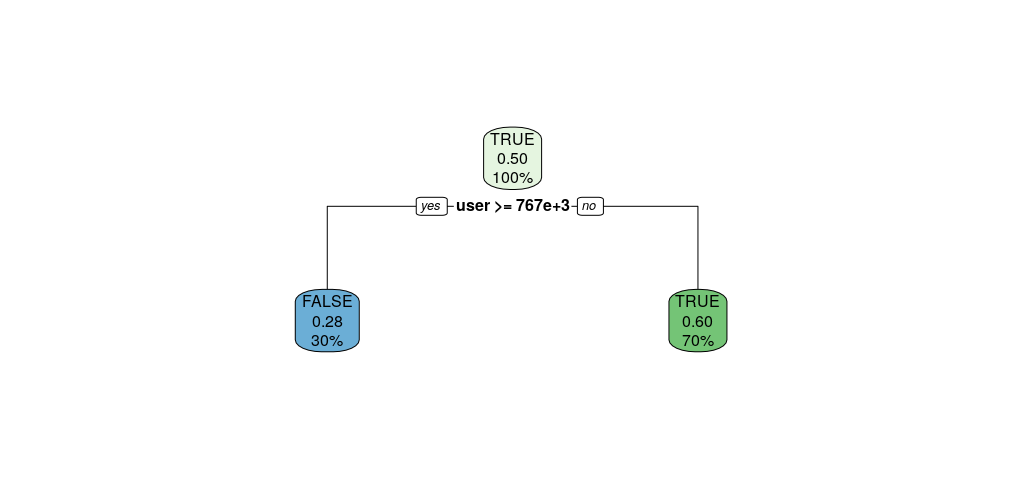
\includegraphics[width=\columnwidth,natwidth=1024,natheight=485]{dtree.png}
  \caption{Prediction tree generated by Decision Tree model}\label{fig:dtree}
\end{figure}
Figure~\ref{fig:dtree} shows generated tree by Decision Tree model. The tree simply differentiates samples by their user's id by a threshold value, which is too simple to be applicable.\newline
	The next approach we tried was General Linear model, which uses binomial distribution for regression and logit function for linking. This model is the best choice within this research scope because it produced a predictor with reasonable coefficients, and its implementation is latterly shown to heavily depend on a matrix equation whose calculation can be accelerated by GPU hardware. Moreover, this model also performs as well as Decision Tree model does with relatively low False Acceptance Rate and False Rejection Rate. In following subsection, this model is used for optimization. The model evaluation result will be described in result section in detail.
\subsection{Other approach}
 Visualization technique like PCA and t-SNE in~\cite{maaten2008visualizing} have also been applied. By visualization, we can extract most important information from input features by taking their linear (with PCA) or nonlinear (with t-SNE) combinations, then present them by 3, 4 components. In other words, visualization is one of compression method to compress original data into smaller dimension space with least information lost as possible. After the compression, 3 features of the compressed data were taken to make graph to give us general look of the data. From the graph, we may intuitively make assumption on data shape, clusters number, density of each cluster. However, eventually their final result was not good enough, thus they will not be included in detail in this paper.
\section{Optimization}
General Linear model was chosen to be optimized with GPU acceleration. General Linear model is a algorithm whose running time mostly concentrates on least squares solver in multiple iterations. R implementation solves the least squares equation via QR decomposition with Householder reflection, which make the algorithm computational complexity be \(O(m \times n ^ 2 \times k)\) where m is number of samples, n is number of features, and \(k\) is number of iteration until convergence.\newline
Firstly, R's standard General Linear model training process was profiled line by line by profvis package. Figure~\ref{fig:profvis} shows profiled result.\newline
\begin{figure}[ht]
  \vspace*{-1cm}
  \centering
  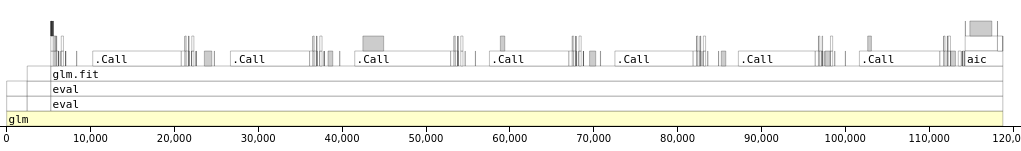
\includegraphics[width=\columnwidth,natwidth=1021,natheight=151]{profvis.png}
  \caption{R General Linear model profiling result}\label{fig:profvis}
\end{figure}
\newline
Longer bar presents longer time it takes to finish the call. The very bottom bar, glm, presents the most outer call be triggered at command line. Subsequently, 2 eval calls were processed as wrapper functions to generalize the algorithm. Glm.fit is the fitting function that iterates a loop to modify coefficient vector until converged. Each iteration calls a \texttt{.Call} subroutine, which is the most intensive code portion and is written in C. Figure~\ref{fig:wrapping} illustrates the program flow. It also denotes that glm.fit subroutine takes 93.42\% of glm call and \texttt{.Call} subroutine takes the majority 58.13\% running time of glm.fit in all iterations. This implies that optimizing the bottleneck \texttt{.Call} subroutine will make it possible to speed up the algorithm by at most 2.2 times. Although 2.2 times speed up upper bound is not a much gain, the optimization on this subroutine is mandatory and a basis for subsequent development on eliminating iteration overhead.\newline
\begin{figure}[ht]
  \vspace*{-2.5cm}
  \centering
  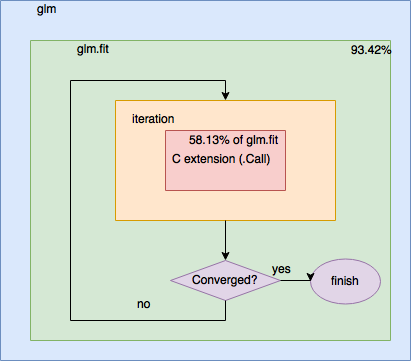
\includegraphics[width=\columnwidth,natwidth=411,natheight=362]{wrapping.png}
  \caption{General Linear model trainer program flow chart}\label{fig:wrapping}
\end{figure}
\newline
 What C extension does is calling R's standard stats package's \texttt{C\_Cdqrls} internal C function to solve Least Squares Linear equation, i.e.\ to find solution vector x which satisfies
  \[x = argmin_x(|Ax - b|)\]
A matrix's dimension is proportional to the model input, and is 9,064,492 records by 27 features. A's 27 columns presents 26 input features and 1 additional intercept feature (free coefficient). \texttt{b} presents target label feature. \texttt{C\_Cdqrls} is a C wrapper of a popular and canonical FORTRAN version of high performance computing mathematical library named linpack with slight modification to optimize QR decomposition when processing linearly dependent columns. This library is notably optimized while still maintaining its generalization and correctness.\newline
Our optimization focuses on porting this external C program to make use of GPU power. Similar to the standard library implementation, it takes 3 steps to solve the least squares linear equation. Assume A is a matrix of m rows by n columns. First, A matrix is decomposed into form \(A = QR\) such that \(Q\) is unitary matrix of size \(m\), \(R\) is upper right triangular matrix of \(m\) row by \(n\) column. Next, reassign b by setting \(b \vcentcolon= t(Q) \times b\) where \(t(Q)\) is transpose of matrix \(Q\). And then evaluate final solution x via backward substitution such that Rx = b to take advantage of R being upper right triangular matrix. All 3 steps are available in CUDA Toolkit CUSOLVER library version 9.1 to directly use GPU acceleration for the calculation. However, in step 1 CUDA Toolkit CUSOLVER library does not support non linearly dependent columns input matrix. We investigated 2 ways to go through this barrier. First way is to run QR decomposition algorithm twice, one to detect and eliminate linearly dependent columns, and another to execute QR decomposition on linearly independent columns matrix. This version of optimization is called \texttt{CUSOLVER LS solver}. In second way, manual QR decomposition was conducted via Householder reflection, combined with linearly dependent columns removal in decomposition. This version of optimization is called \texttt{manual LS solver}. QR decomposition via Householder algorithm with its variance are described is described in~\cite{Kerr:2009:QDG:1513895.1513904}. The most simple version of the algorithm in this paper was adopted with slight modification to detect linearly dependent columns. When calculating Householder reflection matrix of a column, we check if its norm is greater than a value, namely tolerance value, if it is not greater than this threshold, this column will be moved into end of the matrix followed with previously calculated elements on the same column. At time of being written,~\cite{Kerr:2009:QDG:1513895.1513904} was believed that it is the fastest announced QR implementation executing entirely on the GPU~\cite{Kerr:2009:QDG:1513895.1513904}. In future development, we will investigate modifying this algorithm to achieve better overall result.\newline
 Figure~\ref{fig:qr_flow} describes CUSOLVER LS solver and manual LS solver programs' flow\newline
\begin{figure}[ht]
  \vspace*{-3.6cm}
  \centering
  
\includegraphics[width=\columnwidth,natwidth=451,natheight=548]{qr_flow.png}
  \caption{Least Squares Linear solvers program flow}\label{fig:qr_flow}
\end{figure}
\newline
It is also worthwhile to mention that converged condition checking does not require all data of linear solver to be copied back from GPU device memory to Host memory. However, due to time frame of the research, the implementation still relies much on R's standard implementation. In future development, this redundant copy removal should take high priority.\newline
All 3 programs and R standard program were set to use same tolerance setting and their results were cross checked to make sure they execute same number of iterations and produce similar result. Execution time of overall model trainer and total execution time in all iterations of C external call were recorded to make comparison. \texttt{nvprof} was also used to evaluate GPU performance and each subroutine's contribution on overall program. R standard program is speeded up by openblas shared library with number of OMP thread be 1. Various number of OMP threads setting was also measured to check OMP effect onto the algorithm.\newline
Because of high portion of overhead timing and particular shape of input matrix, 3 version of C extensions were laterly profiled.
\section{Result}
 This section includes 2 subsections which illustrates selected model's accuracy and how much the optimization accelerate the algorithm. It is worthwhile to mention that model evaluation use 70\% data set for training and remaining 30\% for testing while optimization does use all data set for benchmark result.
\section{Model evaluation}
 Trained General Linear model can predict correctly 78.71\% test data while False Acceptance Rate and False Rejection Rate were 10.69\% and 10.60\% respectively.
\begin{center}
  \begin{equation}
    \notag
    \begin{aligned}
      \text{Correctness} &= \frac{\text{Number of correctly predicted test samples}}{\text{number of test samples}} \\
      &= \frac{2,140,394}{2,719,348}=78.71\%
    \end{aligned}
  \end{equation}
\end{center}
\begin{center}
  \begin{equation}
    \notag
    \begin{aligned}
      \text{False Acceptance Rate} &= \frac{\text{number of accepted negative test samples}}{\text{number of test samples}} \\
      &= \frac{290,583}{2,719,348}=10.69\%
    \end{aligned}
  \end{equation}
\end{center}
\begin{center}
  \begin{equation}
    \notag
    \begin{aligned}
      \text{False Rejection Rate} &= \frac{\text{number of rejected positive test samples}}{\text{number of test samples}} \\
      &= \frac{288,371}{2,719,348}=10.60\%
    \end{aligned}
  \end{equation}
\end{center}
\begin{figure}[ht]
  \vspace*{-2.5cm}
  \centering
  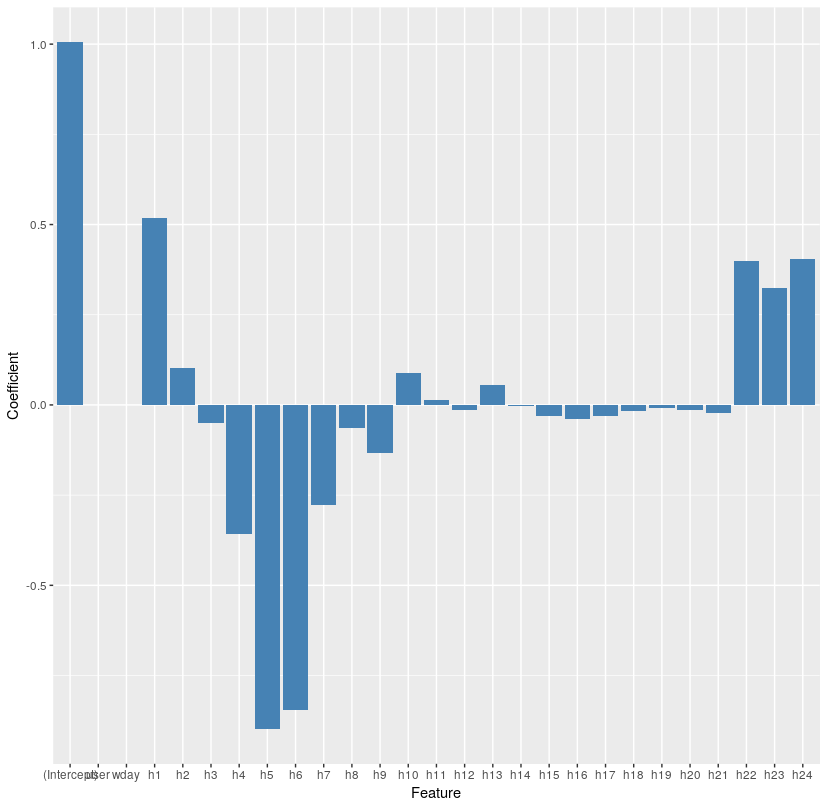
\includegraphics[width=\columnwidth,natwidth=827,natheight=805]{glm_coef.png}
  \caption{Trained General Linear model's coefficients}\label{fig:glm_coef}
\end{figure}
 According to Figure~\ref{fig:glm_coef}, trained General Linear model's coefficients of \(h_4, h_5, h_6\) have high absolute value to compensate its low numerical value compared to other features, as illustrated from Figure~\ref{fig:access_mean}. On the other hand, \(h_{22}, h_{23}, h_{24}, h_1\) features' coefficients have high absolute numerical to emphasize their diversity in our sample. This can be observed from Figure~\ref{fig:access_var} where these features' variances are relatively higher than the others.\newline

\begin{figure}[ht]
  \vspace*{-2.5cm}
  \centering
  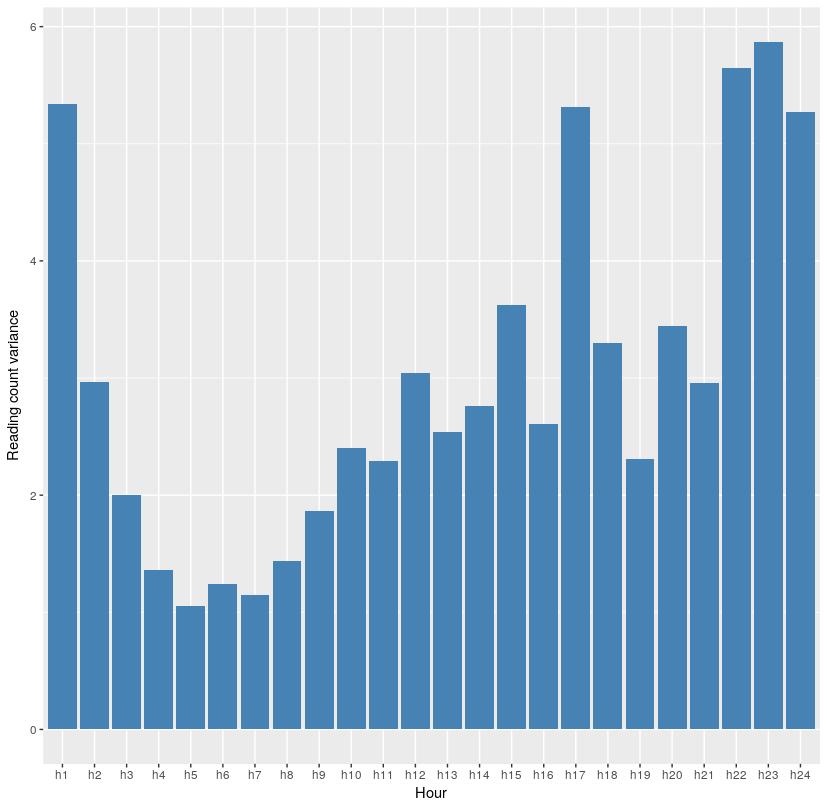
\includegraphics[width=\columnwidth,natwidth=827,natheight=805]{access_var.png}
  \caption{Access count variance each hour in a day}\label{fig:access_var}
\end{figure}
\begin{figure}[ht]
  \vspace*{-1.5cm}
  \centering
  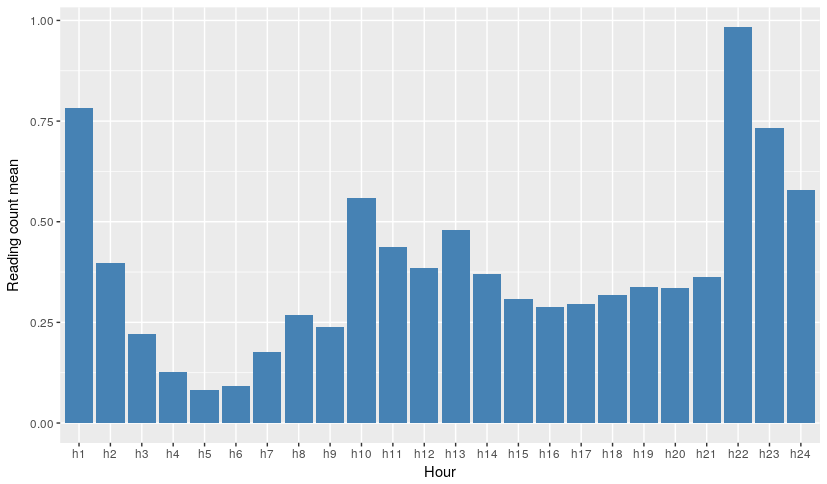
\includegraphics[width=\columnwidth,natwidth=827,natheight=484]{access_mean.png}
  \caption{Mean number of reading by hour in a day}\label{fig:access_mean}
\end{figure}
\section{Optimization}
Time for training all data with standard R algorithm, manual LS solver and CUSOLVER LS solver were 112.79 seconds, 87.579 seconds, 88.897 seconds respectively. These timing result is described in detail in Figure~\ref{fig:qr_ret}\newline

\begin{figure}[ht]
  \vspace*{-1.5cm}
  \centering
  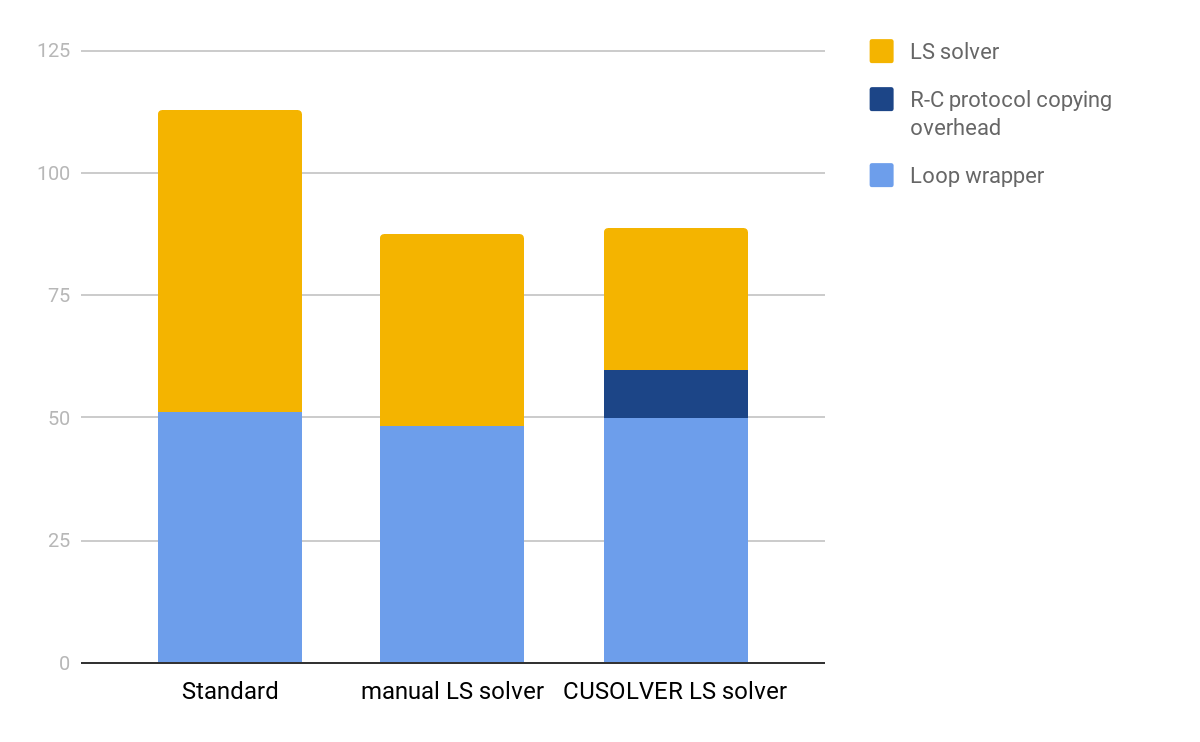
\includegraphics[width=\columnwidth,natwidth=1200,natheight=742]{qr_ret.png}
  \caption{Training time of 3 implementation3}\label{fig:qr_ret}
\end{figure}
Figure~\ref{fig:qr_ret} shows that CUSOLVER LS solver C extension run 2.12 times faster than R standard version \texttt{C\_Cdqrls}. Because of the major portion of overhead timing, the overall algorithm can speed up merely 1.27 times over maximal ideal speed up rate of 2.2 times. C extension running time of CUSOLVER LS solver is slightly faster than manual LS solver's one. This can be explained by the fact that input matrix is indeed linearly independent, CUSOLVER LS solver implementation only need to run QR decomposition once without caring about linear independence while manual LS solver version does care about. In CUSOLVER LS solver running time, there exists portion named \texttt{R-C protocol copying overhead}. This is time occupied by memory transfer between R program and C extension because CUSOLVER LS solver program does not use optimized interface while manual LS solver does. This portion elimination can be adopted with not much effort.\newline

\begin{figure}[ht]
  \vspace*{-2cm}
  \centering
  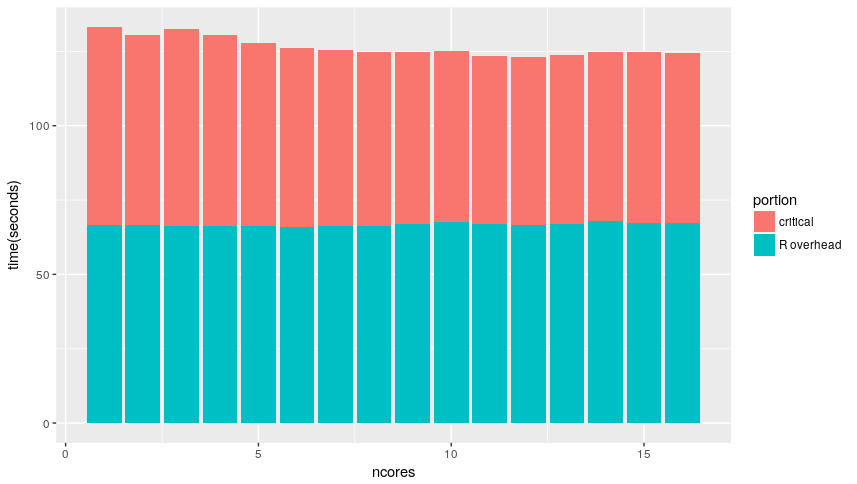
\includegraphics[width=\columnwidth,natwidth=857,natheight=484]{qr_blas_ret.png}
  \caption{Relation between BLAS accelerated run time with number of OMP cores}\label{fig:qr_blas_ret}
\end{figure}

 According to Figure~\ref{fig:qr_blas_ret}, there is no strong relation between number of OMP threads and algorithm performance. Probably, R's extension \texttt{C\_Cdqrls} is not compiled with OpenMP\@. Before going to a solid conclusion, an experiment on CPU usage measurement of training algorithm was done by using Linux htop tool. Number of OpenMP threads was set to be 16, same with number of machine's physical cores. Figure~\ref{fig:htop} indicates a timing when htop catches a moment that all CPUs are fully used. However, the phenomenon disappeared immediately. This shows the fact that the training algorithm does not execute parallel well enough. The same experiment also was done to the C extension \texttt{C\_Cdqrls}. Eventually, there was no moment that more than 1 CPU is fully used. This opens an interesting topic for future research on parallelizing the training algorithm.\newline

\begin{figure}[ht]
  \vspace*{-1cm}
  \centering
  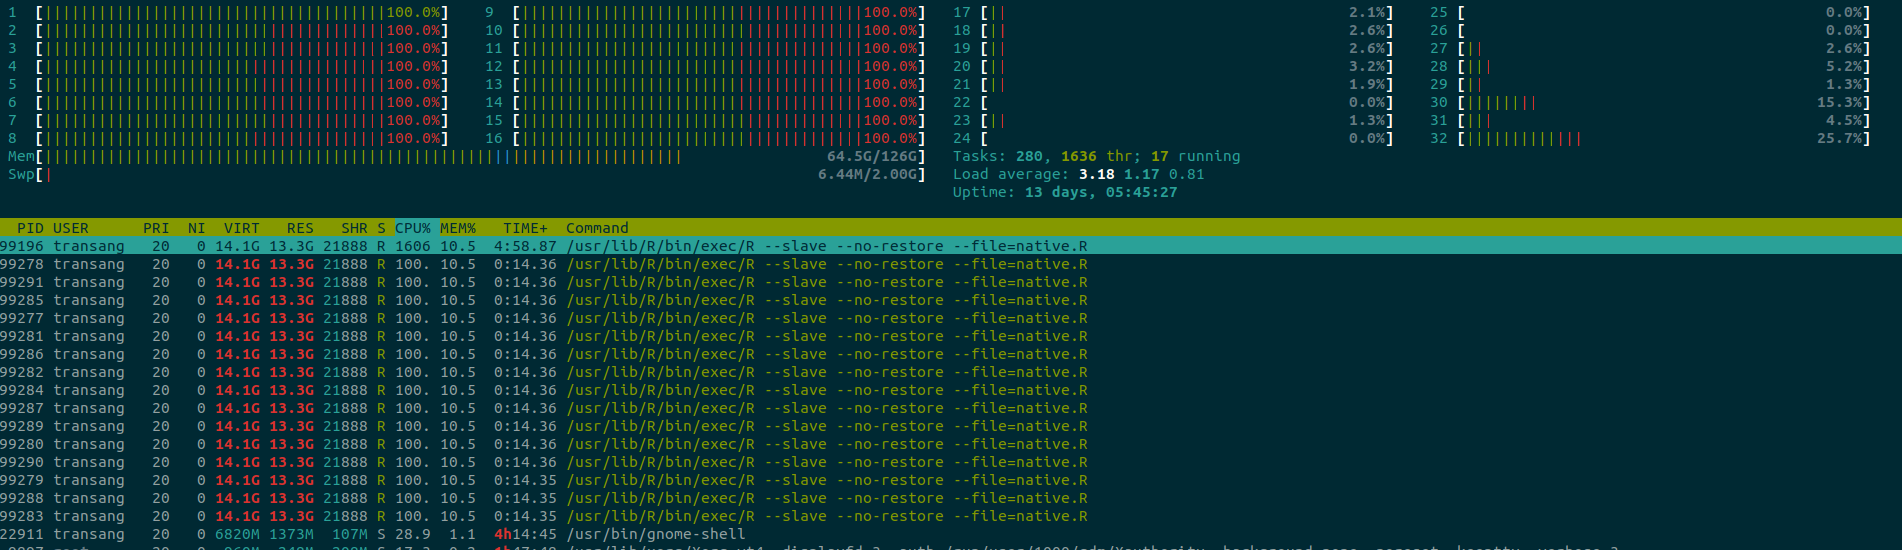
\includegraphics[width=\columnwidth,natwidth=1902,natheight=550]{htop.png}
  \caption{htop catches a glimpse when all CPUs are fully used}\label{fig:htop}
\end{figure}

\begin{figure}[ht]
  \vspace*{-2cm}
  \centering
  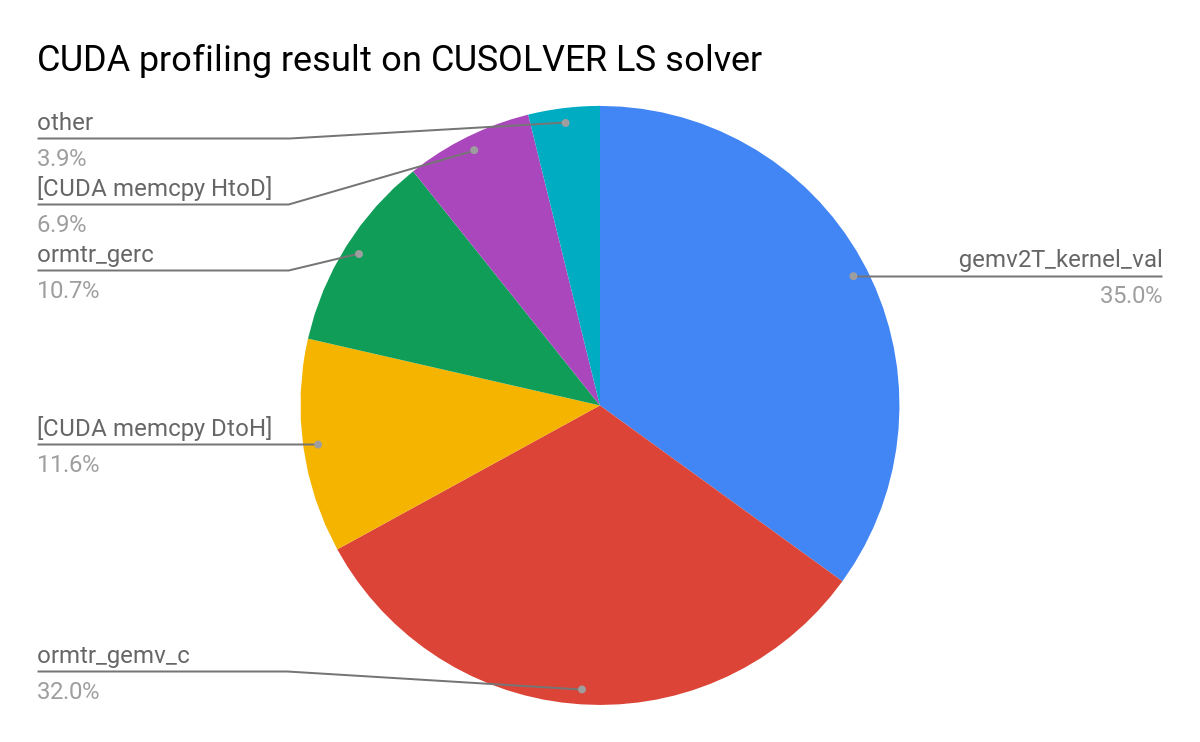
\includegraphics[width=\columnwidth,natwidth=1200,natheight=742]{nvprof_qr.png}
  \caption{GPU profiling result via nvprof of CUSOLVER LS solver}\label{fig:nvprof_qr}
\end{figure}

\begin{figure}[ht]
  \vspace*{-2cm}
  \centering
  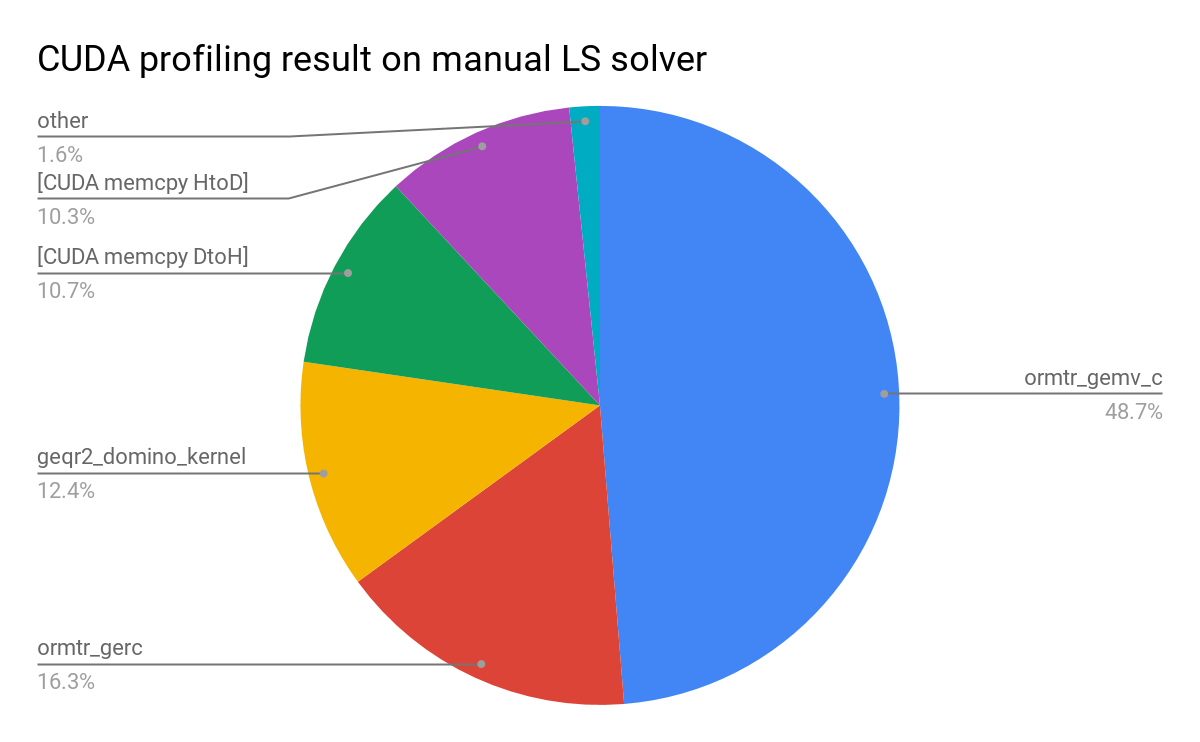
\includegraphics[width=\columnwidth,natwidth=1200,natheight=742]{nvprof_manual.png}
  \caption{GPU profiling result via nvprof of manual LS solver}\label{fig:nvprof_manual}
\end{figure}
From Figure~\ref{fig:nvprof_qr} and Figure~\ref{fig:nvprof_manual}, we can observe that CUDA memcpy routine, a memory transfer routine between CPU (host) and GPU (device), takes around 20\% of the execution on GPU device. This proves the potential of time reduction in future because in current implementation, all data is copied back to CPU after each iteration for convergence check while actually only a small portion of data is required.\newline

\begin{figure}[ht]
  \vspace*{-2.2cm}
  \centering
  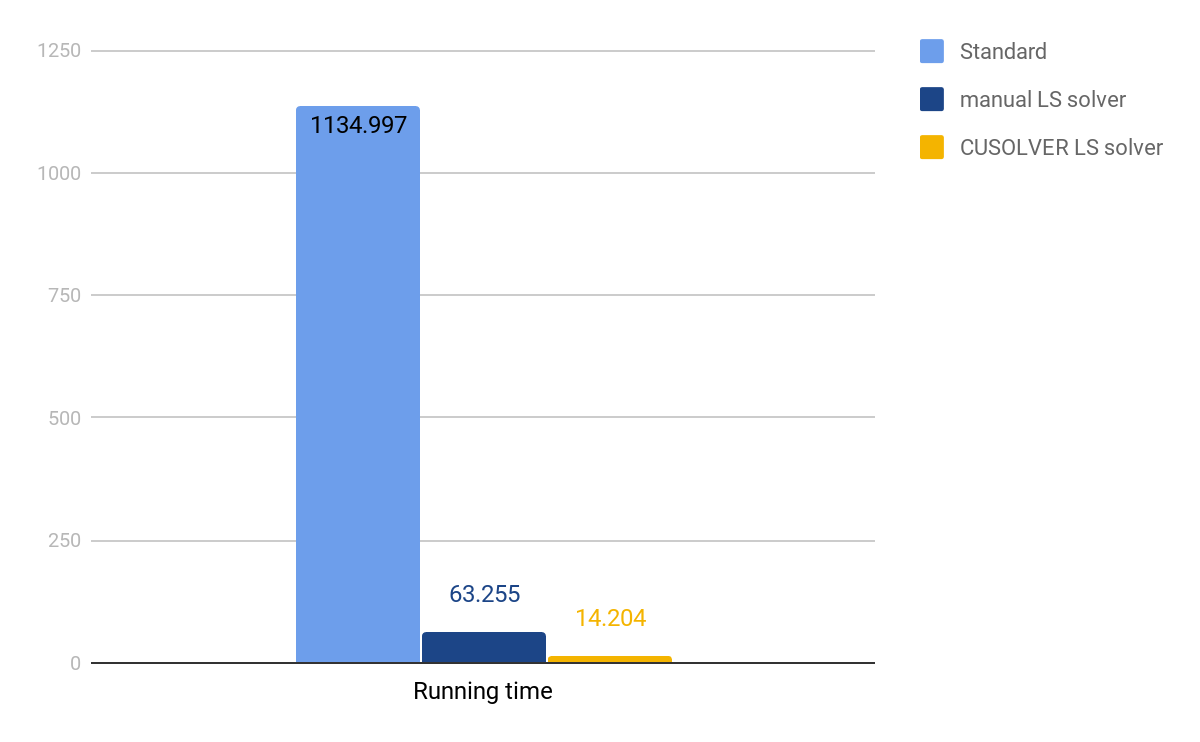
\includegraphics[width=\columnwidth,natwidth=1200,natheight=742]{c_square.png}
  \caption{Isolated C extension time comparison on 3000 rows by 2000 columns matrix}\label{fig:c_square}
\end{figure}

\begin{figure}[ht]
  \vspace*{-1.5cm}
  \centering
  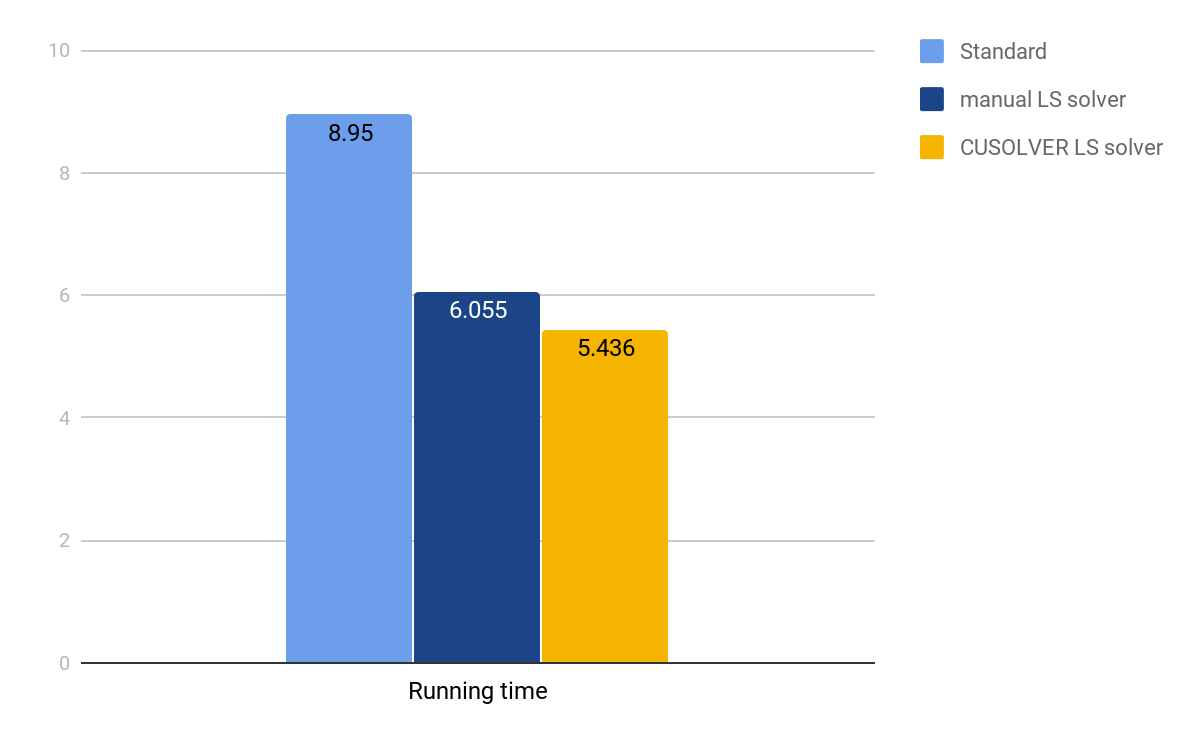
\includegraphics[width=\columnwidth,natwidth=1200,natheight=742]{c_narrow.png}
  \caption{Isolated C extension time comparison on 9,064,492 rows by 27 columns matrix}\label{fig:c_narrow}
\end{figure}
Figure~\ref{fig:c_square} and Figure~\ref{fig:c_narrow} emphasize matrix dimension's effect on C extension performance. With input matrix of 3,000 rows by 2,000 columns, GPU version speeded up LS solver by 17.94 times and 79.91 times resepectively. While with input matrix of 9,064,492 rows by 27 columns their speedup rate were merely 1.48 times and 1.65 times respectively. This implies that narrow matrix does not take more advantage of GPU speedup than square matrix.
\section{Conclusion}
Comparing with R. Kobayashi's result in~\cite{kobayashi1}. General Linear model in this paper decreases both False Acceptance Rate and False Rejection Rate by 1.14 times (from 12.15\% down to 10.69\%) and 1.3 times (from 14.0\% down to 10.60\%) respectively, although these results slightly depends on model choice and false sample generation method. As discussed in methodology section, graph based approach is very promising. If it is well developed, it will not only be helpful on user classification and distinguishment but also has potential on content recommendation system. For example: user next reading chapter suggestion predictor.\newline
Due to major timing fraction of overhead timing, the optimized version of training algorithm achieved relatively high speedup of 1.27 times under 2.2 times upper bound limit. This speedup can be improved much more with convergence check improvement by reducing almost of memory transfer between GPU device and CPU host in middle iterations. The memory transfer should be done only in the first and the last iteration. Last experiment of the research proved that CUDA speedup effect highly depends on input matrix shape. That is to say, the more features input model has the more speedup this research's optimization gains. It is significant to take notice that both Least Squares solver implementations were not fully optimized. CUSOLVER LS solver requires calling QR decomposition twice due to CUDA Toolkit CUSOLVER library's low abstraction. On the other hand, manual LS solver is nothing more than a simple linear QR decomposition with Householder reflection. Blocked Householder QR algorithm in~\cite{Kerr:2009:QDG:1513895.1513904} is one of the fastest QR implementations executing entirely on the GPU~\cite{Kerr:2009:QDG:1513895.1513904}, with some more investigation on capability with linearly dependent system, it is clearly applicable and gains much speedup. In contrast to GPU optimization technique, it is worthwhile to take attention on multicore optimization by installing and loading appropriate lapack library to exploit multicore power.\newline
The last benchmark result on isolated C extension performance proves GPU accelerated algorithm's effectiveness to wide matrix. That is to say the accelerated algorithm gains more speedup on model with high number of features. Especially, when training model with categorical variables expanded, number of features increases proportionally to categorical variables' domain.

\bibliographystyle{plain}
\bibliography{myref_paper}

\end{document}
